\chapter{Numerical Model}
\begin{multicols}{2}
%\begin{lstlisting}[language=Python, caption=Python example]
%def incmatrix(genl1,genl2):
%    m = len(genl1)
%    return M
%\end{lstlisting}
\section{Model Development}
Auricchio and Pettrini \cite{auricchio2004three} give a method for developing a three-dimensional model for stress-induced tranformation in SMAs in discrete and continuous time cases. We will briefly discuss the development of their continuous-time model, which is based on the methods described in Section \ref{sec:FED}. It is important to note that this model assumes only small strains in the material. This is acceptable because even in large deformations, oftentimes only small strains are induced. The model's constitutive relations are thermodynamically consistent, as they satisfy the second law of thermodynamics; in particular, the form common in continuum mechanics expressed by the Clausius-Duheim inequality,
\begin{align}
    D:=D_\mathrm{me}+D_\mathrm{th}\geq0.\label{eq:secondlaw}
\end{align}
Equation (\ref{eq:secondlaw}) dictates that the total mechanical and thermal dissipation $D$, (the specific internal entropy production) is necessarily greater than zero.\cite{smith2005smart}
%\todo[color=yellow]{probably need to cite this}
% the math command $\et$ is defined in ._styles.sty

The strain $\varepsilon$ and absolute temperature $T$ are used as control variables. The transformation tensor, $\et$, describes the strain induced by phase transformations of the material. The free energy density function $\psi$ for a polycrystalline SMA can be decomposed to get the following terms (as described in Equations (\ref{eq:freeenergy}) and (\ref{eq:6})):
\begin{itemize}
    \item The elastic strain energy from material deformation, defined as
    \begin{align}
    \psi_\mathrm{el}=\frac{K}{2}v^2+G\norm{\vb{e}-\et}^2-3\alpha Kv(T-T_0).
    \end{align}
    As in Section \ref{sec:FED}, $K$ is the bulk modulus, $v$ is the volumetric strain (as in Equation \ref{eq:5}), $G$ the shear modulus, $\alpha$ the coefficient of thermal expansion, and $T_0$ an initial temperature.
    \item The chemical energy from martensitic transformation, given by
    \begin{align}
    \psi_\mathrm{ch}=\beta \langle T-M_\mathrm{f}\rangle\norm{\et},
    \end{align}
    where $\beta$ is a coefficient relating the critical stress and temperature. The angled brackets denote that we only consider the positive part of $T-M_\mathrm{f}$ (as described in \cite{auricchio2004three}). In analogy to Equation (\ref{eq:6}), we note here that%\todo{set $T\to\theta$? since that's in \ref{sec:FED}} 
    $f(T):=\beta\langle T-M_\mathrm{f}\rangle$ which depends only on the temperature.
    \item The transformation strain energy,
    \begin{align}
    \psi_\mathrm{tr}=\frac{H}{2}\norm{\et}^2,
    \end{align}
    where $H$ is the hardening parameter mentioned in Section \ref{sec:FED}.
    \item The free energy absorbed or released by a change in temperature (relative to $T_0$),  
    \begin{align}
    \psi_\mathrm{id}=(u_0-T\eta_0)+c\sbr{(T-T_0)-T\ln\frac{T}{T_0}},
    \end{align}
    assuming an ideal incompressible solid, where $c$ is the specific heat capacity, $u_0$ the internal energy at $T_0$, and $\eta_0$ the entropy at $T_0$.
    \item The indicator function $\mathscr{I}(\et)$ defined as in Equation (\ref{eq:indicator}) above.
    %\begin{align}
    %\mathscr{I}(\et)=\begin{cases}
    %0 & \norm{\et}\leq\varepsilon_\mathrm{L},\\
    %\infty & \norm{\et}>\varepsilon_\mathrm{L}.
    %\end{cases}
    %\end{align}
    %This function is set, as we require that $\smash{0\leq\norm{\et}\leq \varepsilon_\mathrm{L}}$, where $\varepsilon_\mathrm{L}$ is a material property: the maximum transformation strain attained by the material in a uniaxial test.
\end{itemize}
Summing all of the above together, we obtain our original convex free energy function,
\begin{align}
    \psi(v,\varepsilon,\et, T)=\psi_\mathrm{el}+\psi_\mathrm{ch}+\psi_\mathrm{tr}+\psi_\mathrm{id}+\mathscr{I}%_{\varepsilon_\mathrm{L}}
    (\et).
\end{align}
We can therefore obtain our four constitutive equations. For the continuous-time model, these are given by
\begin{align}
\begin{split}
    p&=\pdv{\psi}{v}=K\sbr{v-3\alpha(T-T_0)},\\
    \vb{S}_\mathrm{dev}&=\pdv{\psi}{\vb{e}}=2G(\vb{e}-\et),\\
    \eta&=-\pdv{\psi}{T}=\eta_0+3\alpha Kv - \beta\norm{\et}\frac{\langle T-M_\mathrm{f}\rangle}{\abs{T-M_\mathrm{f}}}+c\ln\frac{T}{T_0},\\
    \vb{X}&=-\pdv{\psi}{\et}=\\
    &\phantom{=}\vb{S}_\mathrm{dev}-\sbr{\beta\langle T-M_\mathrm{f}\rangle +H\norm{\et}+\partial \mathscr{I}%_{\varepsilon_L}
    (\et)}\partial\et.\\
    %\gamma&\geq 0,\\
    %\et&=\et_n+\Delta\zeta \pdv{F(\vb{X})}{\mathbf{\bm{\sigma}}},\\
    %\norm{\et}&\leq \varepsilon_\mathrm{L},\\
    %F(\vb{M})&=\sqrt{2J_2}+m\frac{J_3}{J_2}-R\leq0,\\
    %\Delta\zeta&\geq0,\\
    %\Delta\zeta F(\vb{X})&=0.
\end{split}\label{eq:const-rel}
\end{align}
Here, we have that $p$ is the volumetric part of the stress $\bm{\sigma}$ (i.e., pressure), $\vb{S}_\mathrm{dev}$ is the deviatoric part thereof, $\eta$ is the entropy, and the second-order tensor $\vb{X}$ is the thermodynamic force due to strain; a kind of relative stress. The derivatives $\partial \mathscr{I}(\et)$ and $\partial\et$ in the definition of $\vb{X}$ Equation (\ref{eq:const-rel})  are defined in Equation (\ref{eq:derivative2}).
We define the evolution of $\et$ as
\begin{align}
    \dot{\vb{e}}^\mathrm{tr}=\dot\zeta\pdv{F(\vb{X})}{\bm{\sigma}},\label{eq:evolution}
\end{align}
with the Kuhn-Tucker optimality conditions
\begin{align}
    \dot\zeta\geq0, && F\geq0, &&\textrm{and} \quad \dot\zeta F=0.\label{eq:conditions}
\end{align}
The limit function, $F$, is given by\begin{align}
    F(\vb{X})=\sqrt{2J_2}+m\frac{J_3}{J_2}-R,\label{eq:limfunc}
\end{align}
where $m$ is a material parameter, $J_2,J_3$ are invariants of $\vb{X}$ of the second and third order respectively, and $R$ is the radius of elastic domain. 

Equations 
(\ref{eq:const-rel}),
(\ref{eq:evolution}), (\ref{eq:conditions}), and
(\ref{eq:limfunc}), constitute the time-continuous model for the SMA.

\section{Computational SMA Model}
Smith and Massad developed a Homogenized Energy Model for SMAs in Matlab \cite{smith2004model}.
\begin{lstlisting}[language=matlab, caption=Contents of main file]
  m=matparam(1);
  c=comparam(m);
  [sig,ep,T,xm,xp,tspan] = polycryst(0:400,input_Te(0),m,c);
\end{lstlisting}
\subsection{Setup}
The model is first initialized using the provided material parameters in \texttt{matparams.m}. It takes in 19 unique material parameters, some of which include the volume density, specific heat capacity, as well as resistivities, temperatures, thermal expansions, and key temperatures for the martenite and austenite phases.
Out of the box, the code is set up to simulate Nitinol.

 Next, additional key parameters are computed and assigned in the \texttt{comparams.m} script. From these, the model can be developed.

The script \texttt{polycryst.m} sets up the polycrystal homogenization model. This comprises two functions: the first is called \texttt{polycryst}, and the second is \texttt{integrand}. 
\begin{lstlisting}[language=matlab, caption=Polycryst function parameters]
function [sig,ep,T,xm,xp,tspan] = polycryst(tspan,Tini,mparams,cparams)
\end{lstlisting}
The first input parameter (\texttt{tspan}) is chosen to be the range from 0 to 400 discrete seconds. This is long enough to obtain a full hysteresis loop in the generated plots. The input temperature is calculated through another script titled \texttt{input\_Te}, which returns an input temperature based on the current time value. The last two input parameters are simply derived from \texttt{matparams} and \texttt{comparams}. 

\subsection{Algorithm}
Next, the function sets up a double integral computation using a 4-point Gauss-Legendre Quadrature method. Smith describes the method in \cite{smith2005smart} as a method for numerically evaluating integrals over $D=\sbr{-1,1}\cross\sbr{-1,1}$ using Legendre polynomials,
\begin{align}
    P_n(x)=\frac{1}{2^n n!}\dv[n]{}{x} \del{x^2-1}^n,\ n=0,1,2,\ldots
\end{align}
To approximate the integral of a 2-D function $f(x,y)$, we can take the sum
\begin{align}
    \int_a^b\int_c^d f(x,y)\,\mathrm{d}x\mathrm{d}y\approx \sum_{i=1}^{n_x}\sum_{j=1}^{n_y}f(x_i,y_i)w_iw_j,
\end{align}
where $x_i,y_i$ are the roots of the $n\textsuperscript{th}$ Legendre polynomial $P_n$ described above (in this case, we are interested in $P_4$), and $w_i,w_j$ are simply weights which can be obtained from a reference table. In the model SMA code, these constants can be obtained by calling a function in \texttt{gweights.m}. Note that we can do a transformation to set the domain of integration to $\sbr{-1,1}\cross\sbr{-1,1}$ to satisfy the requirements.
\begin{lstlisting}[language=matlab, caption=Snippet of main integrationn loop,label=codecode]
%%Double Integration
tic; 
Fy = zeros(4,length(tspan)); 
FyT=Fy; Fym = Fy;  Fyp = Fy;
funx = Fy; funy=Fy;    funxT = Fy; funyT=Fy;
funxm = Fy; funym=Fy;  funxp = Fy; funyp=Fy;
ep=zeros(size(tspan)); T=ep; xm=ep; xp=ep;
for jy = 1:numsub
    ysub = gnodes(jy,numsub,y0,y1);
    for inodey = 1:4  %y Subintervals
        sigef = ysub(inodey);
        
        %x Integration
        Fx = repmat(0,size(funx));     FxT = repmat(0,size(funxT));
        Fxm = Fx;     Fxp = Fx;
        for jx = 1:numsub
            xsub = gnodes(jx,numsub,x0,x1);
            for inodex = 1:4 %x Subintervals
                dsig = xsub(inodex);
				[ep,T,xm,xp] = integrand(dsig,sigef,tspan,Tini,mparams,cparams,lgmu,lgvar,sevar);
				funx(inodex,:) = ep; 	funxT(inodex,:) = T;
				funxm(inodex,:) = xm;	funxp(inodex,:) = xp;
			end
            Fx = Fx + funx; %4xlength(tspan) Matrix
            FxT = FxT + funxT; %4xlength(tspan) Matrix
			Fxm = Fxm + funxm;  Fxp = Fxp + funxp; 
        end %End x integration
        
        funy(inodey,:) = gw'*Fx; %1xlength(tspan) Vector
        funyT(inodey,:) = gw'*FxT; %1xlength(tspan) Vector
        funym(inodey,:) = gw'*Fxm;  funyp(inodey,:) = gw'*Fxp; 
    end
    Fy = Fy + funy; %4xlength(tspan) Matrix
    FyT = FyT + funyT; %4xlength(tspan) Matrix
	Fym = Fym + funym;  Fyp = Fyp + funyp; 
end
\end{lstlisting}

The code then iterates over each set node to evaluate the energy function integrand, each time recomputing the required parameters, as shown in \ref{codecode}.
\begin{lstlisting}[language=matlab, caption=Integrand function parameters]
function [ep,T,xm,xp] = integrand(dsig,sigef,tspan,Tini,mparams,cparams,lgmu,lgvar,sevar)
\end{lstlisting}
The \texttt{integrand} function is called in this loop to update the integrand. Put simply, the function outputs the strain output vector \texttt{ep}, internal temperature vector \texttt{T}, and the $M^+,M^-$ phase vectors \texttt{xp, xm}. With this, we can recompute our parameters and solve for the energy function.

\subsection{Results}
Finally, the code generates plots of the results using the \texttt{Plotfun.m} script. Four different plots are outputted, seen in Figures \ref{fig:simgraph1} and \ref{fig:simgraph2}. 

The top plot in figure \ref{fig:simgraph1} shows the fraction of the solid in each state (austentite in red and martensite in blue). The lower plot in figure \ref{fig:simgraph1} shows how the temperature of the solid changes as the system evolves in time. The minimum temperature is attained at $t\approx\SI{180}{s}$, when the material is entirely in the martensite state. As the temperature rises agin to a peak, the solid returns to its austenite configuration. Phase transitions occur at the critical stresses $\sigma_M$ and $\sigma_A$, whose values depend on the parameters used. 

The top plot in figure \ref{fig:simgraph2} shows a clear hysteresis loop in the stress-strain curve. The material begins at minimum stress and strain in the bottom left. Initially, as the stress increases, so does the strain with it. Once the critical strain is reached, we see the hysteretic behaviours begin to appear. 

\end{multicols}
\vspace{30pt}
\begin{figure}[ht]
\begin{minipage}{0.48\textwidth}
    \centering
    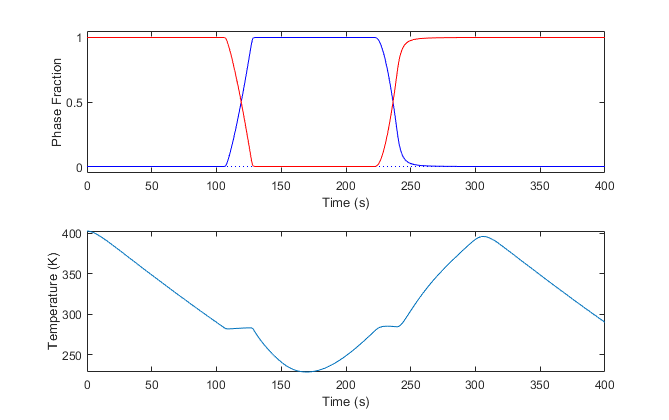
\includegraphics[width=\textwidth]{._figures/graphphases.png}
    \caption[Plots generated by SMA code in Matlab]{Temperature evolution of the system in time (top). Proportion of the solid in \textcolor{red}{austentite} and \textcolor{blue!50!black}{martensite} phases (bottom).}
    \label{fig:simgraph1}
\end{minipage}\hfill
\begin{minipage}{0.48\textwidth}
    \centering
    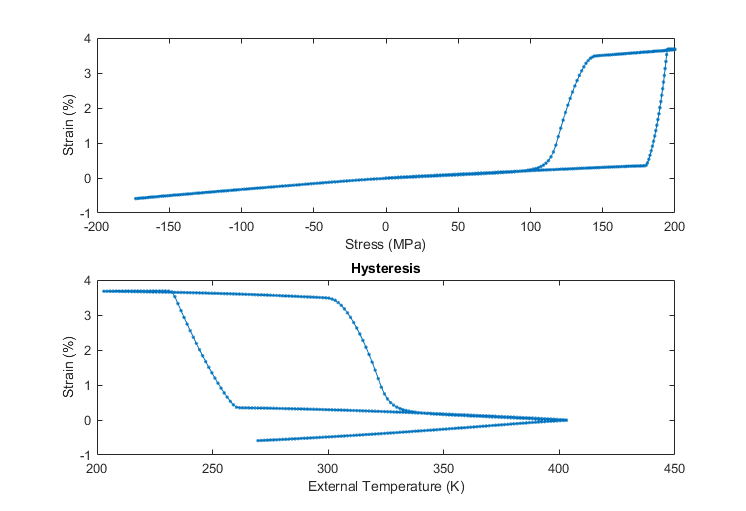
\includegraphics[width=\textwidth]{._figures/stressstrain.png}
    \caption[Stress-strain curve generated by SMA code in Matlab]{Stress-strain and temperature-strain curves generated by the SMA model for Nitinol. Both curves clearly show hysteretic behaviour.}
    \label{fig:simgraph2}
\end{minipage}
\end{figure}